%\section{Results}

The QE-like differential cross section~\cite{supplemental} as a function of 
\QSqproton is shown in Fig.~\ref{fig:cross_section_model_overlay_POT} (top), 
along with predictions from the \genie and \nuwro~\cite{Nowak:2006xv,Golan:2013jtj} 
generators using a RFG model. Several extensions to the 
\nuwro QE RFG prediction are shown, inspired by measurements 
based on lepton kinematics. Each prediction represents the sum over all 
reactions with at least one $>$110~MeV proton and no pions in 
the final state. The inelastic contributions to this QE-like cross section  
from the \genie (dark dashed) and \nuwro (light dashed) predictions 
are shown, and differ in both rate and shape. For both generators, 
the inelastic component is dominated by $\Delta(1232)$ production and decay, 
where the pion is absorbed by the residual nucleus. 

The shape of \xsecproton can be compared between prediction
and data with reduced systematic uncertainty by normalizing each
prediction to the data. Figure~\ref{fig:cross_section_model_overlay_POT} (bottom) 
shows the ratio between the data and normalized prediction to the \genie
RFG prediction. For both the absolute and the shape comparisons, the $\chi^2$ 
between the data and each prediction, including correlations between bins, 
is given in Table~\ref{tab:model_compare}. The highest \QSqproton data point
contributes mostly to the total $\chi^2$ for the \genie RFG and \nuwro RFG 
with RPA+Nieves. The remaining predictions get most of their
total $\chi^2$ from the middle data points, which have higher
and positive covariance values, but these predictions visibly have an opposite 
trend to the data.

%%%%%%%%%%%%%% figure set 3 %%%%%%%%%%%%%%%%
\begin{figure}[htpb]
\centering
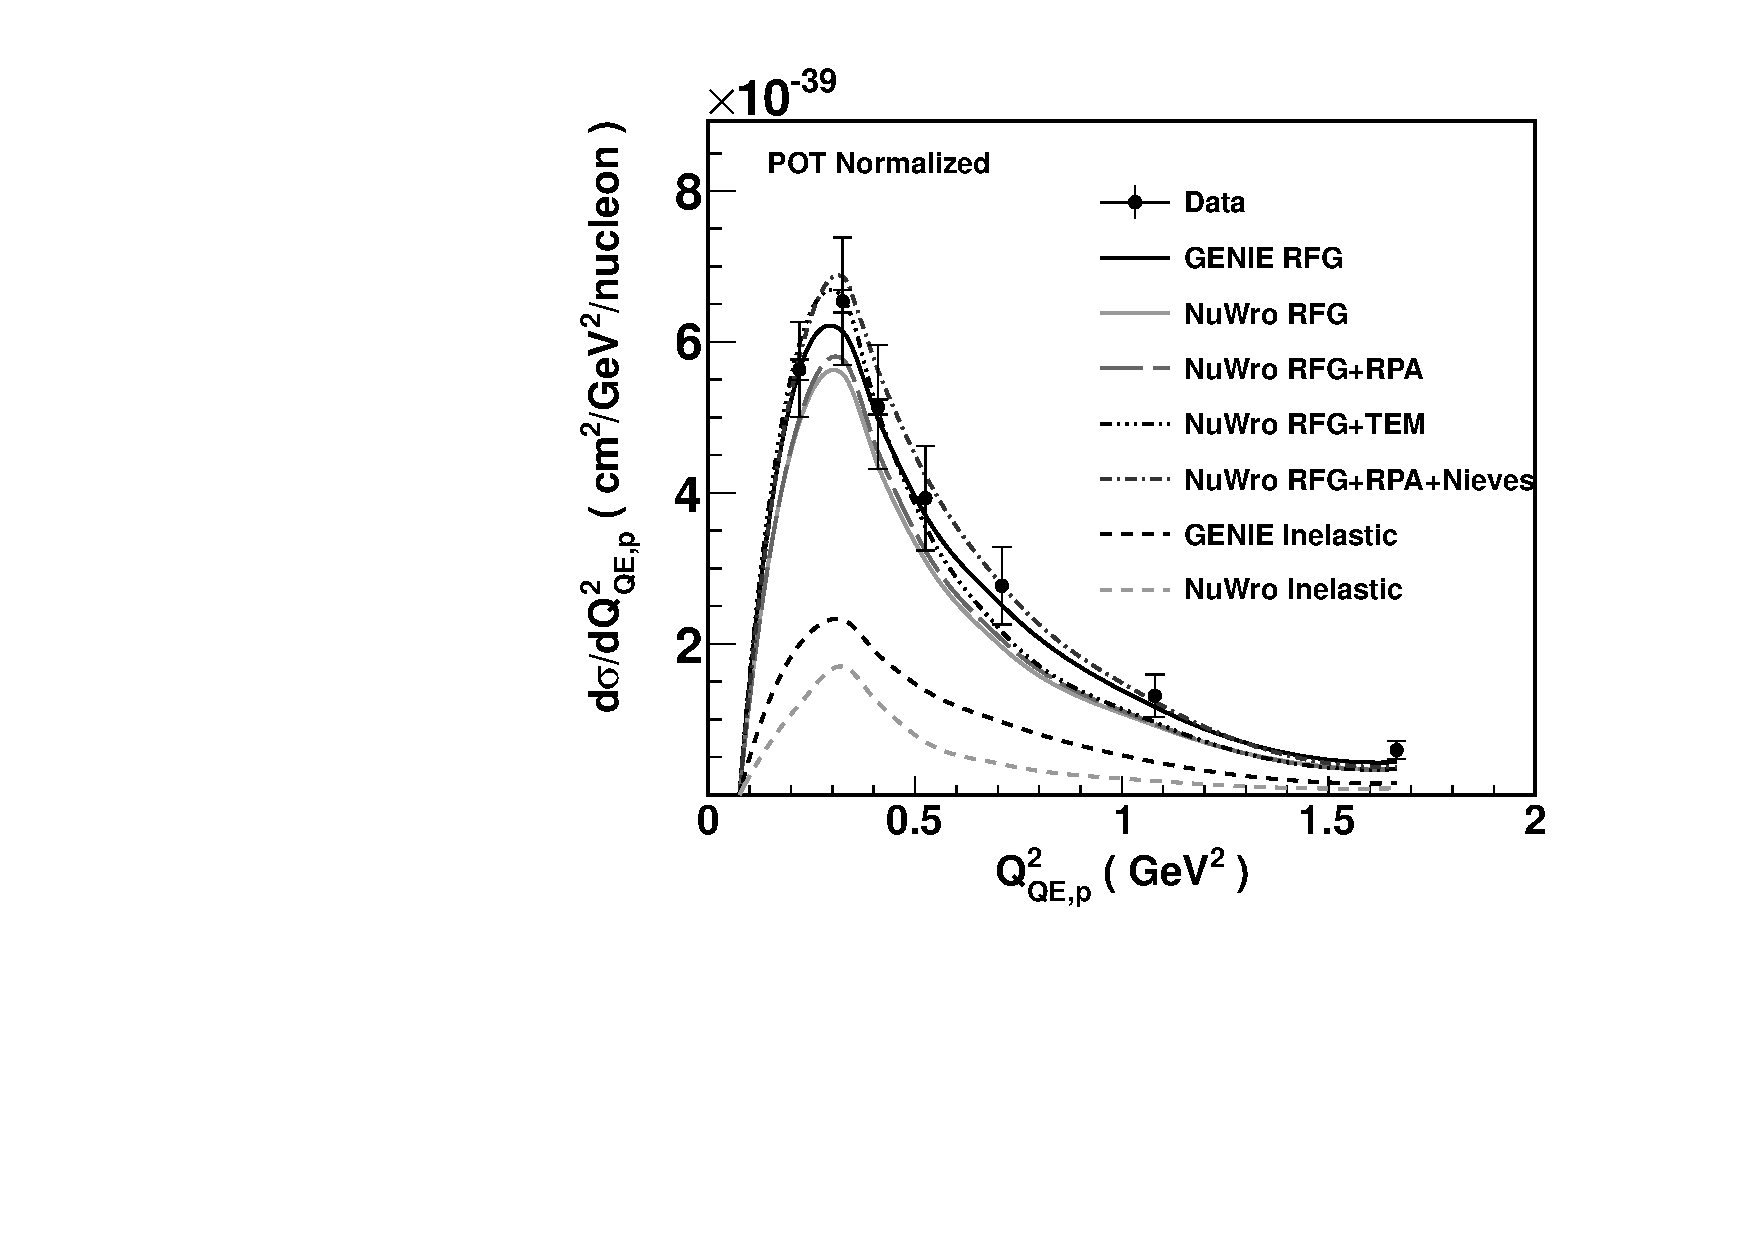
\includegraphics[width=\columnwidth]{figures/h_proton_q2_xsection_overlay_pot.pdf}
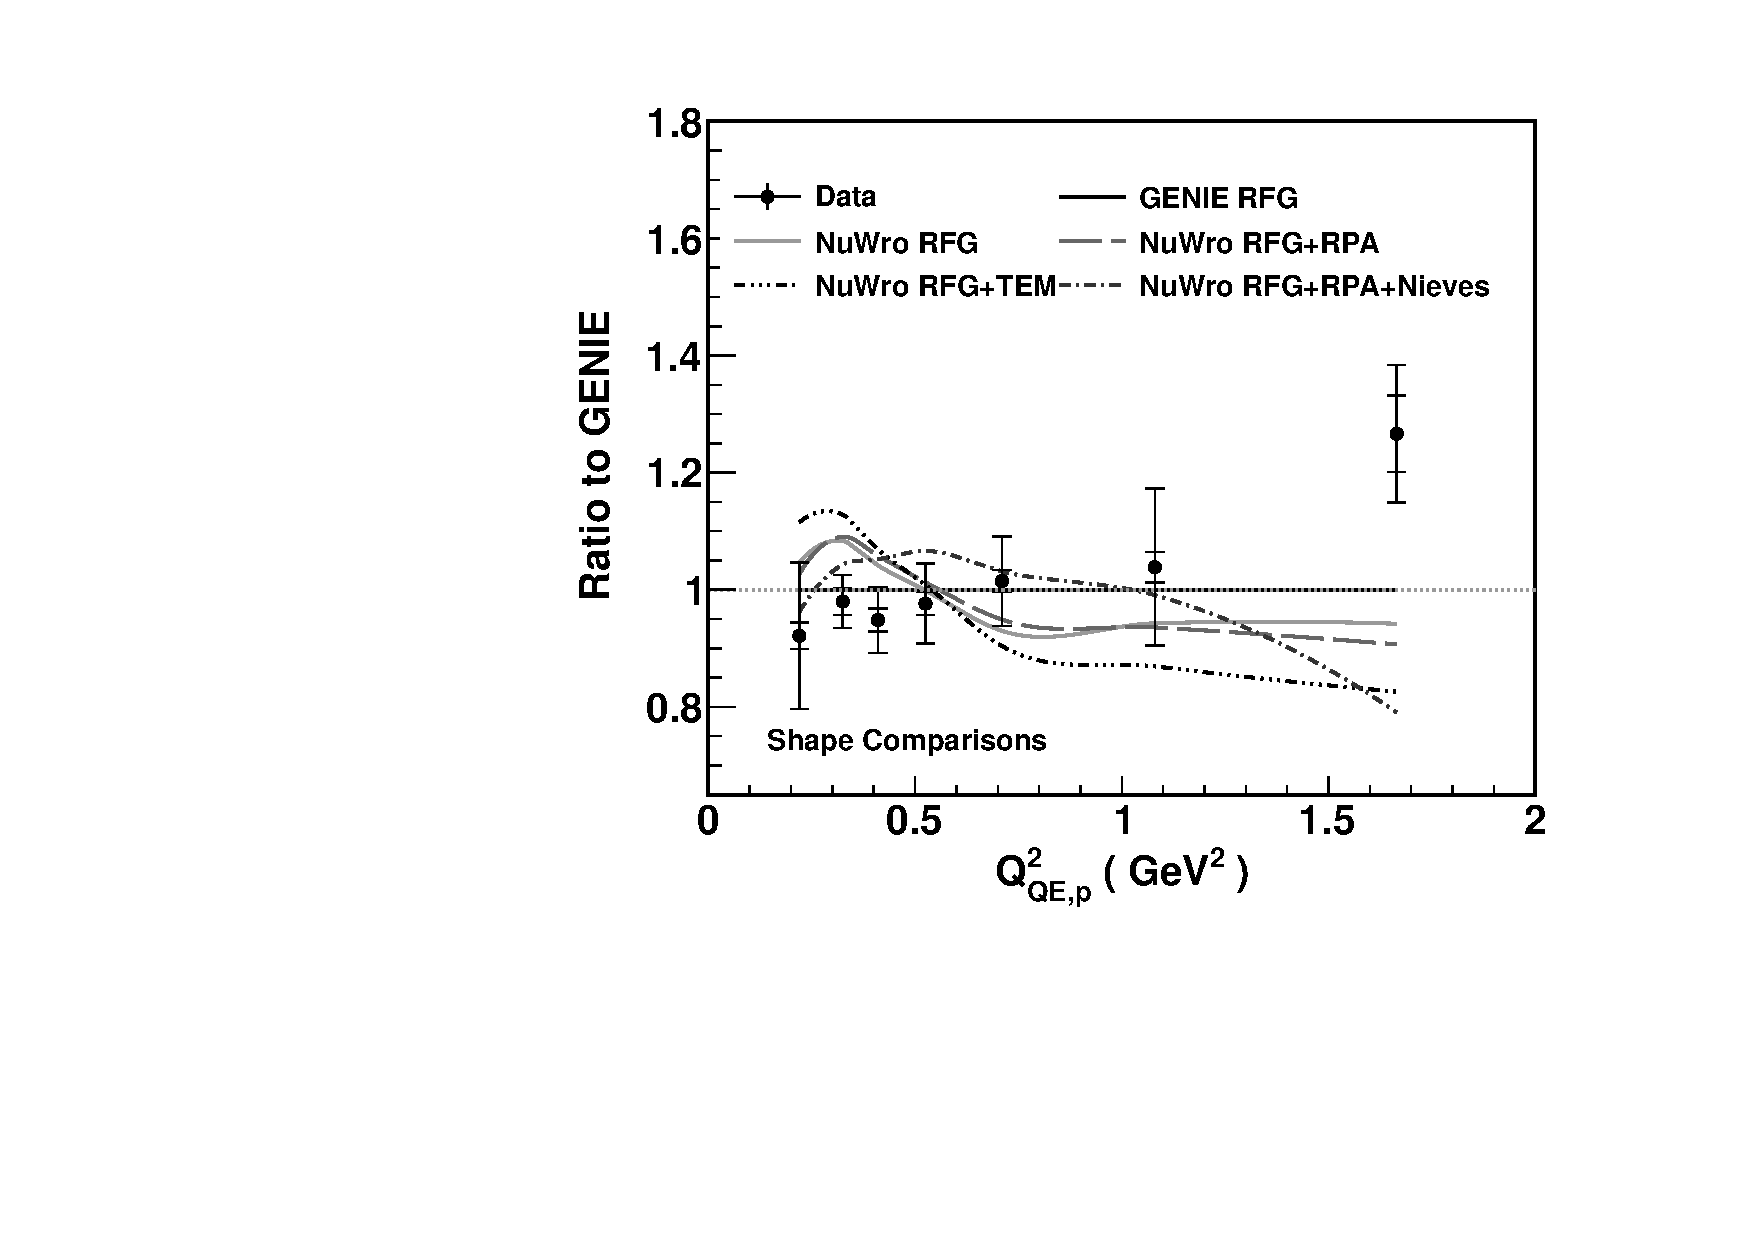
\includegraphics[width=\columnwidth]{figures/h_proton_q2_xsection_ratio_area.pdf}
\caption{(Top) QE-like cross section versus \QSqproton compared to several different 
predictions, along with the \genie (dark dashed line) and \nuwro (light dashed line) 
predictions of the inelastic contribution to the QE-like prediction.
(Bottom) Ratio between the data and predictions to the \genie RFG prediction including the 
inelastic component, where all models are normalized to the data.  
The inner (outer) error bars correspond to the 
statistical (total) uncertainties.}
\label{fig:cross_section_model_overlay_POT}
\end{figure}
%%%%%%%%%%%%%%%%%%%%%%%%%%%%%%%%%%%%%%%%

The rate and shape of the data are best described by the \genie RFG model 
with the inelastic component, followed 
by the \nuwro RFG model with its very different prediction of the 
inelastic process. The remaining \nuwro predictions 
become more discrepant with the shape of the data, as various implementations 
of nuclear effects are incorporated. 

\genie and \nuwro calculate QE scattering using the independent 
nucleon impulse approximation, 
%as prescribed by Smith and Moniz~\cite{Smith:1972xh}, 
the BBBA2005 parameterization~\cite{Bradford:2006yz} 
of the vector form factors, and an axial mass of $0.99~\rm GeV/c^2$. 
As described above, \genie has in addition an approximation of short-range 
correlations included 
%by adding a high-momentum component to the 
%momentum spectrum of initial-state nucleons 
as prescribed by Bodek-Ritchie~\cite{Bodek:1980ar,Bodek:1981wr}. 


\begin{table}[!htbp]
\centering
\caption{Calculated $\chi^{2}$ between the data and various models with M$_{A}$ = 0.99~GeV/c$^{2}$. 
The number of degrees of freedom is 7 (6) for the rate (shape).\label{tab:model_compare}}
\scalebox{0.8}
{
\begin{tabular}{ l c c }
Model & Rate $\chi^{2}$   & Shape $\chi^{2}$ \\ \hline
\genie RFG                &   8.5  &  10.8 \\
\nuwro RFG                &  12.2  &  19.9 \\
\nuwro RFG + RPA          &  13.5  &  21.7 \\
\nuwro RFG + RPA + Nieves &  25.9  &  28.5 \\
\nuwro RFG + TEM          &  27.6  &  34.5 \\
\end{tabular}
}
\end{table}

The difference between \genie and \nuwro RFG predictions arises primarily in
the difference between the two simulations' treatments of inelastic scattering.
In \genie, resonance production is defined using the formalism of 
Rein-Sehgal~\cite{Rein:1980wg} while in \nuwro, 
it is defined as interactions with invariant hadronic mass $W <$~1.6~GeV, 
and where contributions come from $\Delta(1232)$ 
excitations. \genie and \nuwro handle interactions with $W >$~1.6~GeV similarly 
and transport hadrons through the nucleus using different implementations of 
an intranuclear cascade model. 

RPA calculations predict a suppression of the cross section at very low \QSq 
from long-range correlations, and enhancement at moderate \QSq 
due to short-range correlations. For the \nuwro RPA 
calculation~\cite{Graczyk:2003ru}, the suppression happens below \minerva's proton 
kinetic energy threshold, and its curve is nearly identical to \nuwro RFG 
prediction as shown in Fig.~\ref{fig:cross_section_model_overlay_POT}.
MEC between nucleons enhance the cross section and populate the transition 
region between the QE and $\Delta$ peaks. MEC are part of 
both the microscopic model of Nieves~\cite{Nieves:2004wx,Gran:2013kda} and 
the Transverse Enhancement Model (TEM) which is empirically extracted from 
electron scattering data~\cite{Bodek:2011ps}. TEM is based on QE 
lepton kinematics so that the energy transfer follows from reweighting QE events 
rather than filling the transition region between the QE and $\Delta$ peaks, while the Nieves 
model gives systematically higher energy transfers which translate to an enhancement 
at higher proton energies. The proton kinematics are not explicitly calculated  
in either the TEM or the Nieves model, and in NuWro are assigned as described in 
Refs.~\cite{Sobczyk:2012ms,Golan:2013jtj}.

The agreement between the presented QE-like data and the \genie prediction
is in stark contrast to that of the \minerva QE 
measurements~\cite{Fields:2013zhk,Fiorentini:2013ezn}, where \QSq is based on 
muon kinematics and the backgrounds from all inelastic events 
are subtracted. To check the consistency between 
\minerva muon-based QE and proton-based QE-like measurements, the subsample of 
events with muons that are tracked in \minos is used to measure the pure QE 
differential cross section~\cite{supplemental} as a function of \QSq estimated 
from the muon kinematics as given in Ref~\cite{Fiorentini:2013ezn}. 
These results are consistent with the reported QE measurement~\cite{Fiorentini:2013ezn} 
while using a factor of three more protons on target but lower acceptance because 
of the proton track requirement.

The inconsistency of the models of the hadronic and leptonic aspects of the
QE-like sample may be resolved by modifying the $\Delta(1232)$ production cross section and 
nuclear absorption models. Supporting evidence comes from the results of 
the background tuning described above and \minerva's inclusive pion production
measurement~\cite{Eberly:2014mra},which finds $\Delta$-dominated single pion production 
to be nearly 30\% less than the \genie prediction. Refinements to models of multinucleon 
effects, beyond those implemented in these versions of \genie and \nuwro, may 
also resolve the discrepancies seen here.  

This proton-based \xsecproton measurement provides a new way to evaluate the 
modeling of all contributions to the QE-like cross section, and finds that the 
models which best describe the proton kinematics of this interaction differ
from those that best describe the muon kinematics. The models used by 
neutrino oscillation experiments must ultimately reproduce the hadronic as well as 
leptonic kinematics since both affect neutrino energy reconstruction.


 




